%TODO:
%* Finalize list of figures
%* Make figures with different colors
%* Some stats and take-home points from human data
%* Figure out if we want to include complex goals or only simple goals (correlations more or less the same)
%* Include model comparison stats (with no arousal goal, overall correlation = 0.75, and valence correlation = 0.79 (as opposed to 0.96 with arousal)). Just using prior, correlation for state = 0.78
%* Add model result for irony ratings
%* Finalize discussion
%* Fix abstract

% 
% Annual Cognitive Science Conference
% Sample LaTeX Paper -- Proceedings Format
% 

% Original : Ashwin Ram (ashwin@cc.gatech.edu)       04/01/1994
% Modified : Johanna Moore (jmoore@cs.pitt.edu)      03/17/1995
% Modified : David Noelle (noelle@ucsd.edu)          03/15/1996
% Modified : Pat Langley (langley@cs.stanford.edu)   01/26/1997
% Latex2e corrections by Ramin Charles Nakisa        01/28/1997 
% Modified : Tina Eliassi-Rad (eliassi@cs.wisc.edu)  01/31/1998
% Modified : Trisha Yannuzzi (trisha@ircs.upenn.edu) 12/28/1999 (in process)
% Modified : Mary Ellen Foster (M.E.Foster@ed.ac.uk) 12/11/2000
% Modified : Ken Forbus                              01/23/2004
% Modified : Eli M. Silk (esilk@pitt.edu)            05/24/2005
% Modified : Niels Taatgen (taatgen@cmu.edu)         10/24/2006
% Modified : David Noelle (dnoelle@ucmerced.edu)     11/19/2014

%% Change "letterpaper" in the following line to "a4paper" if you must.

\documentclass[10pt,letterpaper]{article}

\usepackage{cogsci}
\usepackage{pslatex}
\usepackage{apacite}
\usepackage{graphicx}
\usepackage{amssymb,amsfonts,amsmath}
\usepackage{todonotes}
\usepackage{caption}
\usepackage{subcaption}
\usepackage{url}

\title{Let's talk (ironically) about the weather: A computational model of verbal irony}
 
  \author{{\large {\bf Justine T. Kao} (justinek@stanford.edu)}, {\large {\bf Noah D.~Goodman} (ngoodman@stanford.edu)}\\
  Department of Psychology, Stanford University}

\begin{document}

\maketitle


\begin{abstract}
Verbal irony plays an important role in how we communicate and express our opinions about the world. While there exist many interesting theories and empirical findings about how people use and understand verbal irony, there is to our knowledge no formal model of how people incorporate shared background knowledge and linguistic information to communicate ironically. Here we present two behavioral experiments that examine people's interpretations of utterances given different contexts. We then describe a computational model that reasons about background knowledge, affect, and the speaker's communicate goals to interpret ironic utterances and their rich affective subtexts. We show that by accounting for two types of affect goals---valence and arousal---our model produces interpretations that closely match humans'. Finally, we discuss the implications of our model on informal theories of irony and its relationship to other types of nonliteral language understanding.


\textbf{Keywords:} 
irony; computational modeling; pragmatics; nonliteral language understanding
\end{abstract}


\section{Introduction}
%\todo[inline]{RDH: Intro is great! Highly readable and makes the point of the paper very clear, even though I'm not super familiar with the literature on irony}
For better or for worse, verbal irony---defined as utterances whose apparent meanings are opposite in polarity to the speaker's intended meaning \cite{roberts1994people, colston2000contrast}---is a major figurative trope of our time. From popular sitcoms to political satire to \emph{\#sarcasm} on Twitter and casual conversations among friends, verbal irony plays an important role in how we communicate and express  opinions about the world. The prevalence of verbal irony poses a puzzle for theories of language understanding: Why would speakers ever use an utterance to communicate its opposite meaning, and how can listeners appropriately interpret such an utterance? Previous work has shown that verbal irony serves several important communicative goals, such as to heighten or soften criticism \cite{colston1997salting}, elicit emotional reactions \cite{leggitt2000emotional}, highlight group membership \cite{gibbs2000irony}, and express affective attitudes \cite{colston1998you, colston1997ve}. These findings suggest that while ironic statements are false under their literal meanings, they are often highly informative with respect to social and affective meanings. 
In this paper we argue that a computational approach previously shown to explain hyperbole \cite{kao2014nonliteral} can also explain irony---once extended to a richer space of affective subtext. 
%In this paper, we present a computational model and behavioral experiments to show that people may use inferences about these alternative dimensions of meaning and the speaker's communicative goals to understand ironic utterances.  

%\todo[inline]{RDH: maybe say \emph{which} alternative dimensions of meaning you'll be focusing on, to set up the distinction you make with the hyperbole model later? Right now, it looks like `alternative' means `social and affective,' but that's not exactly the set of dimensions you use later, right?}

Linguists and psychologists have proposed several informal theories of how people understand verbal irony. According to a classic Grician analysis, listeners first need to recognize that an ironic utterance blatantly violates the maxim of quality (to be truthful); they then arrive at a conversational implicature that the intended meaning is contrary to the utterance's literal meaning \cite{grice20134, wilson2006pragmatics}. While Grice's account is appealing in its treatment of verbal irony as arising naturally from conversational maxims, it does not provide a detailed or satisfactory explanation for how the appropriate implicature is derived from these maxims, or why it is ever rational to deliver an utterance that is opposite from the truth \cite{wilson2006pragmatics}. 
%\todo[inline] {RDH: Maybe give a quick, succinct reason this fails? I don't see the problem\dots but maybe it's not worth the space and I should just read the Wilson paper ;)}
On the other hand, previous work suggests that it is possible and indeed desirable to consider some cases of nonliteral language understanding as a product of general principals of communication, such as reasoning about informativeness with respect to the speaker's communicative goals \cite{kao2014nonliteral, kao2014formalizing}. It is tempting to think that verbal irony can be addressed similarly, and with similar formal precision.
%In particular, a model that reasons about the speaker's affect is able to arrive at the correct, weaker, interpretation of hyperbolic utterances and infer the appropriate affective subtext \cite{kao2014nonliteral}. Many researchers believe that hyperbole and irony are closely related phenomena (cite); we suggest that similar formal principles may account for both. Our goal in this paper is to identify these communicative principles and provide a precise formal account of how they interact to produce ironic interpretations.

Rational Speech Act (RSA) models are a family of computational models that formalize language understanding as recursive reasoning between speaker and listener, and have been shown to account for many phenomena in pragmatics \cite{frank2012predicting, goodman2013knowledge}. \citeA{kao2014nonliteral} introduces a critical extension to basic RSA models by considering the idea that listeners may be uncertain which question under discussion (QUD -- or topic of conversation) the speaker aims to address when formulating an utterance. The listener then must infer the QUD as well as the speaker's intended meaning. For example, a speaker may want to communicate negative affect about a situation (e.g. unhappiness about the cool temperature outside) instead of the precise situation (the temperature outside), in which case choosing an exaggerated utterance (``It's freezing outside!") effectively addresses the QUD. A listener who reasons about the speaker and QUD is then able to use his background knowledge about temperatures to correctly infer that the speaker is upset about the temperature, but that it is unlikely to be literally freezing outside (especially if she is in California). 
%Extending this model to consider QUDs opens up the possibility for a speaker to produce an utterance that is literally false but satisfies her goal to convey affect. 
\citeA{kao2014nonliteral} showed that this model---which we will refer to as qRSA---produces nonliteral interpretations of hyperbolic utterances that closely match humans',  but they considered only a simplified affect space, namely the presence or absence of negative feeling. This overlooks the range of attitudes and emotions that speakers could express with nonliteral utterances. In particular, since verbal irony involves expressing negative meanings with positive utterances and vice versa, a richer space of affect that includes both positive and negative emotions may be key. Here we examine the consequence of considering the range of emotions in an empirically derived affect space within the qRSA model; we show that this minimal change is able to capture many of the rich inferences resulting from verbal irony.


%Here we present a computational model that takes into account common ground and affective dimensions of meaning to model how people understand irony. 

%Since Grice's original proposal, there have been two competing theories of irony understanding: the echoic mention theory \cite{sperber1981irony, jorgensen1984test} and pretense theory \cite{clark1984pretense}. Both theories move away from a straightforward framework of pragmatics. While these informal theories each offer interesting insights into certain aspects of irony, determining which particular theory is superior is beyond the scope of this paper. Instead, we are interested in identifying basic elements of irony that are consistent across different theoretical frameworks and providing a precise formal account of how these elements can be incorporated to produce ironic interpretations. 



%While there are interesting theories and empirical findings about how people use and understand verbal irony, there is to our knowledge no formal model of how people incorporate shared background knowledge and linguistic information to communicate about the world and their attitudes using irony. 

%We observe that across different approaches to verbal irony, researchers agree that common ground between speaker and listener is critical for successful interpretation \cite{williams1984does}. In addition, verbal irony almost always communicates the speaker's attitude about a certain topic (cite). 



In what follows, we will examine interpretations of potentially ironic utterances in an innocuous domain---the weather. We chose the weather as the victim of irony for several reasons. First, people are quite familiar with talking (and complaining) about the weather. Second, we can visually represent the weather to participants with minimal linguistic description in order to obtain measures of nonlinguistic contextual knowledge. Finally, we can vary the weather states to observe how the same utterance is interpreted differently given different contextual knowledge. We first explore how an enriched space of affect impacts the qRSA model, finding the possibility of ironic interpretations. We then present two behavioral experiments that examine people's interpretations of utterances given different weather contexts. We show that by accounting for two types of affect goals, valence and arousal, our model produces interpretations that closely match humans'. Finally, we discuss implications of our model on informal theories of irony and its relationship to other types of nonliteral language understanding.
%\todo{NDG: we do need a mention of other, informal, theories of irony in intro or discussion. if in discussion, say here that we discuss.}

\section{Computational Model}
%Our behavioral experiments confirmed that people's judgments of irony are highly sensitive to their prior knowledge of the world. We also showed that two affective dimensions---valence and arousal---may be especially important for irony. Here we describe an extension to the basic Rational Speech Act (RSA) model that incorporates these elements to produce interpretations of ironic utterances. 


%
%The extended model was able to produce appropriate interpretations of hyperbole as well as its affective subtext. However, since the model only considered a fairly impoverished affect goal (communicating presence or absence of negative affect), it could not take into account cases where a negative utterance is used to communicate positive affect (and vice versa), which is critical in ironic uses (e.g. saying ``Life is so hard!" when sipping iced lemonade on a sunny beach). 
%

In this section, we describe the qRSA model\footnote{See \citeA{kao2014nonliteral} for details and a more leisurely exposition.} and compare different spaces of affect to test the conditions for producing ironic interpretations. 
%
%We begin with a literal listener $L_0$, who interprets all utterances literally. For example, the literal listener will interpret the utterance ``The weather is terrible" to mean that the weather state is \emph{terrible}, and that the speaker has the corresponding negative valence towards the weather. 
%
%Formally, if $u$ is the uttered adjective:
%\[ L_0(s, v, a|u) = \left\{ 
%  \begin{array}{l l}
%    P(v, a | s) & \quad \text{if $s$ = $u$}\\
%    0 & \quad \text{otherwise}
%  \end{array} \right.\]
%where $P(v, a | s)$ is the prior probability that a speaker would feel valence $v$ and arousal $a$ towards the weather state $s$.
%
%We assume that the speaker's goal $g$ is to communicate  along any (or multiple) of the three dimensions of meaning, which results in $2^3 - 1 = 7$ possible goals (the speaker cannot communicate along none of the dimensions). For example, the speaker may want to communicate only the weather state $s$, or only her valence about $s$, or both.
%We assume that the QUD may be about the actual weather, or the speaker's emotional valence towards the weather. 
Following the qRSA model described in \citeA{kao2014nonliteral}, a speaker chooses an utterance that most effectively communicates information regarding the question under discussion (QUD) to a literal listener. We consider a meaning space consisting of the variables $s, A$, where $s$ is the state of the world, and $A$ represents the speaker's (potentially multidimensional) affect towards the state. %\todo{JTK: notation? NDG: seems fine.}
We formalize a QUD as a projection from the full meaning space to the subset of interest to the speaker, which could be $s$ or any of the dimensions of $A$. 
We specify the speaker's utility as information gained by the listener about the topic of interest---the negative surprisal of the true state under the listener's distribution given an utterance, $u$, along the QUD dimension, $q$---leading to the following utility function:
%\todo[inline]{RDH: 1. maybe write out this utility function mathematically? 2. what is the meaning space? Is this just the world space? Or the set of features indexing the world space? 3. maybe explain what the subscripts mean? Using a subscript for $S_1$ sets it up for there to be an $S_2$ or $S_0$, which there isn't!}
%
\begin{equation}
U(u | s, A, q) = \log \sum_{s', A'} \delta_{q(s, A)=q(s', A')} L_{literal}(s, A |u)
\end{equation}
where $L_{literal}$ describes the literal listener, who updates her prior beliefs about $s, A$ by assuming the utterance to be true of $s$. 
The speaker $S$ chooses an utterance according to a softmax decision rule \cite{sutton1998reinforcement}:
$S(u | s, A, q) \propto e^{\lambda U(u | s, A, q)}$,
where $\lambda$ is an optimality parameter.
%
A pragmatic listener $L_{pragmatic}$ then takes into account prior knowledge and his internal model of the speaker to determine the state of the world as well as the speaker's affect. Because $L_{pragmatic}$ is uncertain about the QUD, he marginalizes over the possible QUDs under consideration:
$$
L_{pragmatic}(s, A | u) \propto P(s) P(A | s) \sum_{q}{P (q) S (u|s, A, q)}
$$
%
The resulting distribution over world states and speaker affects is an \emph{interpretation} of the utterance. 

\begin{figure}
\scalebox{0.43}{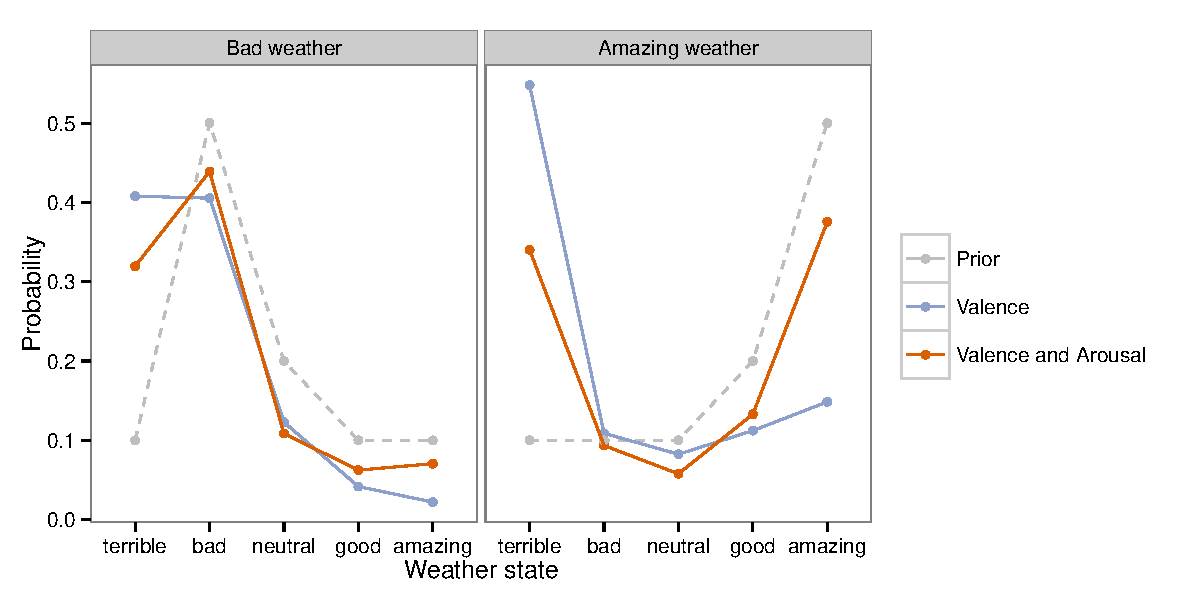
\includegraphics{sim12}}
\caption{Model interpretations of ``The weather is terrible" given different prior beliefs about the weather state and affect dimensions. Gray dotted lines indicate prior beliefs about weather states given a weather context; blue lines indicate interpretations when reasoning only about the speaker's valence; orange lines indicate interpretations when reasoning about both valence and arousal.}
\label{sim12}
\end{figure}
%\todo{NDG: perhaps we could have marker size in fig 1 correspond to interpreted arousal? never mind, we don't have that for the first sim...}

\begin{figure*}
    %\centering
    \begin{subfigure}[b]{0.5\textwidth}
        %\centering
        \includegraphics[width=220pt, height=150pt]{image-grid}
        \caption{The nine weather images shown to participants in Experiments 1 and 2.}
        \label{images}
    \end{subfigure}
    \hfill
    \begin{subfigure}[b]{0.5\textwidth}
       % \centering
        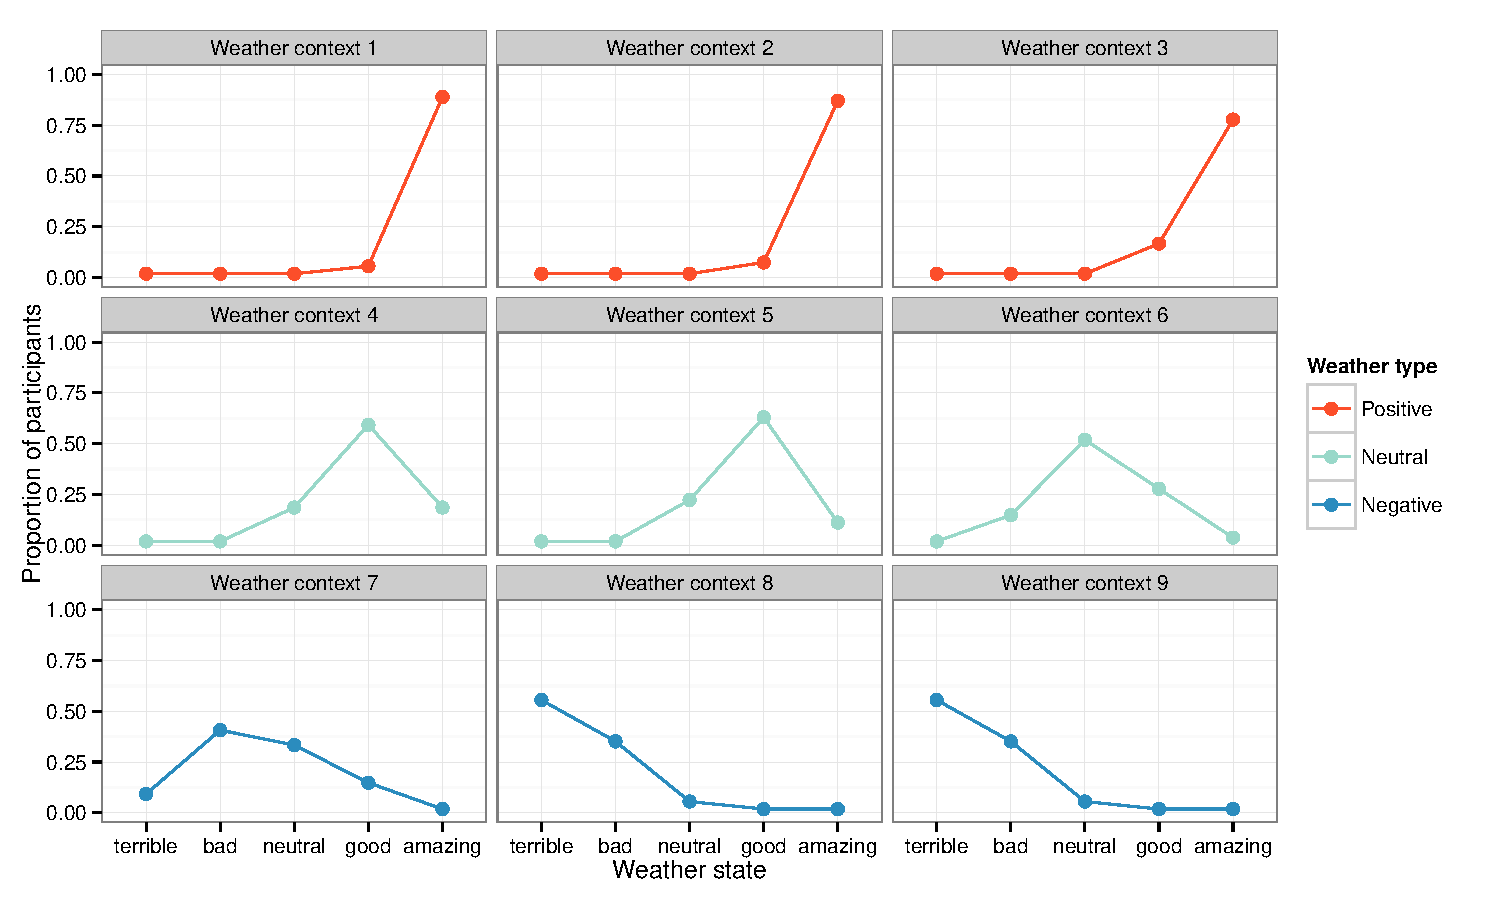
\includegraphics[width=230pt, height=150pt]{priors}
        \caption{The proportion of participants who rated each of the weather contexts as each weather state. 
     %Each panel represents a weather context; each line represents the distribution over weather states for a weather context prior to any linguistic input. For example, the vast majority of participants rated weather context 1 as \emph{amazing}, suggesting that the prior probability of someone believing weather context 1 to be \emph{amazing} is extremely high.
     }
        \label{priors}
    \end{subfigure}
    \caption{Nine weather contexts and their empirically measured priors over weather states.}
    \label{fig:three graphs}
\end{figure*}

%\todo[inline]{RDH: It might be helpful here to point out that you're going to try different ways of specifying the QUD space. Otherwise, it may not be clear what you're `considering' these spaces for.}
%\todo[inline]{NDG: this paragraph is confusing and long-winded. start by describing the assumptions of the simulation: $s$ has five ordered values, consider two different priors corresponding to apparently bad (but not horrible) weather and apparently great weather, consider first qRSA with a single boolean good/neutral $A$. describe the fig 1 result, that we see hyperbole but not irony, without going into the blow-by-blow. then describe the extended $A$ and it's result.}
We performed the following simulations to examine the model's behavior using affect spaces, $A$, that differ in complexity and structure.  
We assume that $s$ has five possible ordered values: \texttt{terrible}, \texttt{bad}, \texttt{neutral}, \texttt{good}, and \texttt{amazing}. We consider two different weather contexts: apparently bad weather and apparently amazing weather, which are each specified by a prior distribution over these states (see gray dotted lines in Figure~\ref{sim12}). We then examine how the model interprets the sentence ``The weather is terrible" in the two weather contexts, given different affect spaces.

We first consider a one-dimensional affect space, where the dimension is emotional valence, and the values are whether the speaker feels negative or positive about the state.  
%
%If $L_1$ thinks it is likely that speaker $S_1$'s goal is to convey negative emotion but believes that it is \emph{a priori} unlikely for the weather state to be \emph{terrible}, he will determine that $S_1$ feels negative about the weather, but that the weather state is more likely less extreme than \emph{terrible}. This produces a hyperbolic interpretation of the utterance. However, if $L_1$ thinks it is \emph{a priori} extremely likely for the weather state to be \emph{amazing}, upon hearing ``The weather is terrible," he will believe that the weather is terrible, because otherwise there is no reason for $S_1$ to choose that utterance. In other words, this model cannot infer a positive state from a negative utterance (and vice versa), thus failing on most cases of verbal irony. 
%
%Suppose there is strong prior belief that the weather state is \texttt{bad}; also suppose that the QUD is the speaker $S$'s emotional valence towards the weather. Based on $S$'s understanding of the literal listener's prior knowledge, she knows that if she produces the utterance ``The weather is terrible," $L_{literal}$ will believe that the weather is \texttt{terrible} and that the speaker is likely to feel negative about it. Since the QUD is successfully addressed if $L_{literal}$ believes that $S$ feels negative towards the weather state, $S$ is motivated to produce the utterance ``The weather is terrible." However, suppose that the pragmatic listener $L_{pragmatic}$ has strong prior belief that the weather state is \texttt{bad}. Since $L_{pragmatic}$ reasons about $S$ and her goals, he realizes that $S$ chose the utterance ``The weather is terrible" to communicate her negative affect and not the true state of the weather. He will then infer that the weather is likely \texttt{bad}, and that $S$ is extremely likely to feel negative towards it, which successfully produces a hyperbolic interpretation. However, suppose there is strong prior belief that the weather is \texttt{amazing}. Given the utterance ``The weather is terrible," $L_{pragmatic}$ interprets it literally to mean that the weather is indeed \texttt{terrible}. This is because if it were \emph{not} terrible, then it would be unlikely for $S$ to choose the utterance, as it is unlikely to communicate either the true state of the world or her valence 
The blue lines in Figure~\ref{sim12} show the model's interpretation of ``The weather is terrible" using this one-dimensional affect space. While the model produces a hyperbolic interpretation (that the weather is \texttt{bad}) given strong prior belief about \texttt{bad} weather, it produces a literal interpretation (that the weather is \texttt{terrible}) given strong prior belief about \texttt{amazing} weather. In other words, a model that only considers valence is unlikely to infer a positive world state from a negative utterance (and vice versa), thus failing on many cases of verbal irony. 

%We now consider a more complex affect space with two dimensions---valence and arousal---to observe its consequence on interpretation. 
Affective science identifies two dimensions, termed valence and arousal, as underlying the slew of emotions that people experience \cite{russell1980circumplex}. 
For example, \emph{anger} is a negative valence and high arousal emotion, while \emph{contentment} is a positive valence and low arousal emotion. 
These two dimensions are not independent, with low arousal implying more neutral valence. 
\todo{JTK: is this non-independence important/necessary to note, or is it confusing?}
%\todo{NDG: is this dependence built into the model's prior? if so, does it matter? if not, we should explore it...} 
Could speakers leverage the arousal dimension to convey high arousal and positive affect (e.g. excitement) using utterances whose literal meanings are associated with high arousal but negative affect (e.g. ``The weather is terrible")? The orange lines in Figure~\ref{sim12} show simulations of the qRSA model with a two-dimensional affect space: whether the speaker feels negative/positive valence and low/high arousal towards the world state. Given strong prior belief that the weather state is \texttt{bad}, the model interprets ``The weather is terrible" to mean that the weather is likely to be \texttt{bad}, again producing a hyperbolic interpretation. However, given strong prior belief that the weather is \texttt{amazing}, the model now places much greater probability on the ironical interpretation of ``The weather is terrible," meaning that the weather is likely \texttt{amazing}. This is because with the enriched two-dimensional affect space, the pragmatic listener realizes that the speaker may be using ``terrible" to communicate high emotional arousal. Note that this result is not simply a straightforward effect of the prior: given the same priors, the model interprets the neutral utterance ``The weather is ok'' as the weather state being \texttt{neutral} and not \texttt{amazing}. %\todo{NDG: is this true?} 
These simulations suggest that a psychologically realistic, two-dimensional affect space enables the model to appropriately interpret ironic utterances in addition to hyperbolic ones. 

%\todo[inline]{NDG: we need to be clearer about what we mean when we say ``one dimensional'' or ``two dimensional'' in the simulations: continuous or discrete? if discrete, are the dimensions binary, or do we have e.g. pos/neutral/neg valence?}



%\todo[inline]{RDH: maybe clarify the distinction between these spaces a bit -- is $a_2$ arousal + valence, while $a_1$ is just valence? It seems counterintuitive that adding \emph{arousal} would give rise to these effects... And not necessarily predicted by previous work?}
%\todo[inline]{JTK: But do we refer to these affect dimensions as valence and arousal? Without first introducing these dimensions with the experiment, how should we talk about them in the model?}


%\begin{figure*}
%\begin{subfigure}{0.5\textwidth}
%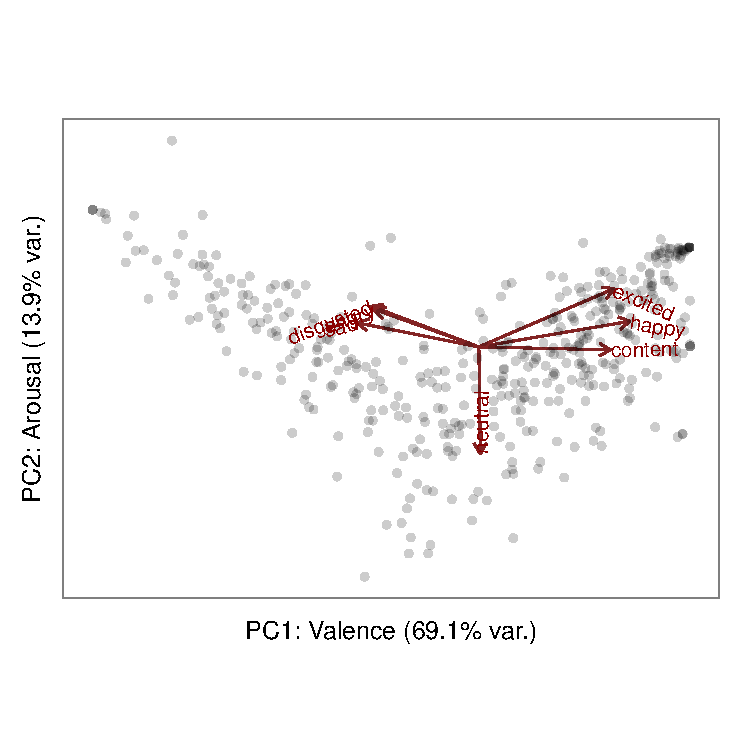
\includegraphics[width=180pt, height=170pt]{biplot.pdf}
%\caption{A biplot of the two principal components of the emotion ratings from Experiment 1. 
%%PC1 corresponds roughly to positive valence, with higher values for \emph{content, happy}, and \emph{excited} and lower values for \emph{sad, angry}, and \emph{disgusted}. PC2 corresponds roughly to high arousal, with higher values for \emph{excited} and {disgusted} than for \emph{content} and \emph{neutral}.
%}
%\label{PCA}
%\end{subfigure}
%\hfill
%\begin{subfigure}{0.5\textwidth}
%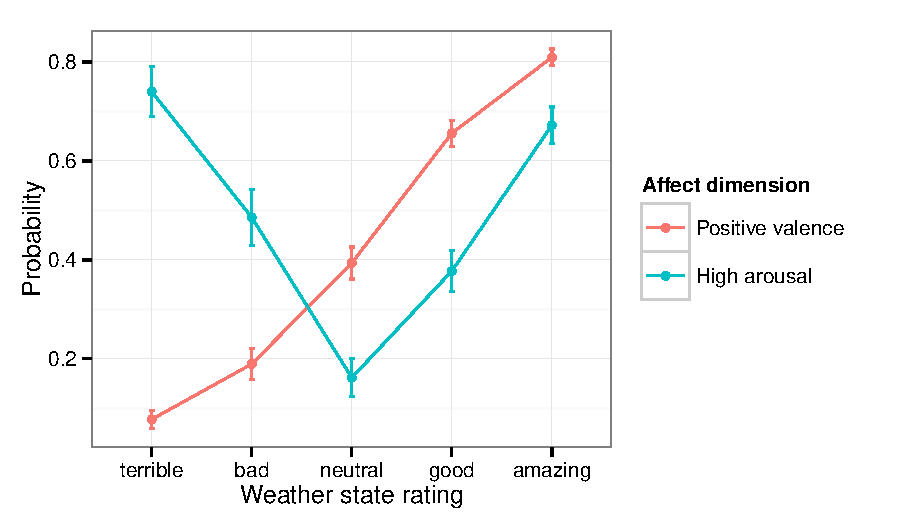
\includegraphics[width=220pt, height=150pt]{affect-prior.pdf}
%\caption{The average probabilities of positive valence and high arousal associated with each weather state. Error bars are $95\%$ confidence intervals.}
%\label{affect-prior}
%\end{subfigure}
%\caption{}
%\end{figure*}

\section{Behavioral Experiments}
In order to quantitatively test the ability of the qRSA model with expanded affect space to capture ironic interpretations, we need appropriate prior distributions, as well as human interpretation data.
We conducted Experiment 1 to measure both prior beliefs over weather states ($P(s)$) for various weather contexts, and the likelihood of various emotions in different weather states (in order to empirically derive the affective space and priors, $P(A | s)$, for this domain).
In Experiment 2, we collected people's ratings of how a speaker perceives and feels about the weather given what she says (e.g. ``The weather is terrible!" when the context clearly depicts sunny weather).

%To produce an interpretation of an utterance in context, the model requires the following input values: (1) $P(s)$: the prior probability of a weather state $s$ given a weather context. (2) $P(A | s)$: the probability of affect $A$ (positive/negative valence and high/low arousal) given a weather state. (3) $P(q)$: the prior probability of a particular QUD (4) The speaker optimality parameter $\lambda$. We derived the values for (1) and (2) from Experiment 1 and fit (3) and (4) to the data from Experiment 2, which we describe below.
%
%In Experiment 1, we measured the prior beliefs over weather states for various weather contexts. We also measured various emotions associated with different weather contexts in order to empirically extract the affective dimensions relevant to this domain. In Experiment 2, we collected people's ratings of how a speaker perceives and feels about the weather given what she says (e.g. ``The weather is terrible!" when the context clearly depicts sunny weather).

%\todo[inline]{I would emphasize in motivating this that we want to explore how the true affective response space can explain irony. Hence we measure the state priors but also measure a bunch of dimensions of potential variance of affect. We can then do dimensionality reduction to extract the true affective dimensions to construct an affect-given-state prior. In model comparison below, make sure we test keeping different numbers of components from the PCA.

%Also make it more clear that the reason to do these experiments is to test a theory of irony understanding, to be described later, that depends on this background knowledge. Maybe the model should go first?}

%We conducted the following two experiments to elicit people's judgements of potentially ironic utterances and their relationship to context and background knowledge. In Experiment 1, we collected participants' ratings of various weather contexts as well as how a person (e.g. Ann) feels about the weather. The weather ratings measure knowledge of the current weather state. The affect ratings measure how people generally feel about different weather states, which captures people's intuitive theory of attitudes towards the weather. In Experiment 2, we collected people's ratings of Ann's judgment of and feelings towards the weather given what she says about it, for example, ``The weather is terrible!" when the weather depicted is clearly sunny and nice.


\subsection{Experiment 1: Prior elicitation}
\subsubsection{Materials and methods}
We selected nine images from Google Images that depict the weather. To cover a range of weather states, three of the images were of sunny weather, three of cloudy weather, and three of rainy or snowy weather. We refer to these images as weather contexts. Figure~\ref{images} shows these nine images.
$49$ native English speakers with IP addresses in the United States were recruited on Amazon's Mechanical Turk. Each participant saw all nine images in random order. In each trial, participants were told that a person (e.g. Ann) looks out the window and sees the view depicted by the image. They then indicated how Ann would rate the weather using a labeled 5-point Likert scale, ranging from \texttt{terrible}, \texttt{bad}, \texttt{neutral}, \texttt{good}, to \texttt{amazing}. Finally, participants used slider bars to rate how likely Ann is to feel each of the following seven emotions about the weather: \emph{excited}, \emph{happy}, \emph{content}, \emph{neutral}, \emph{sad}, \emph{disgusted}, and \emph{angry}, which are common emotion categories \cite{ekman1992argument}\footnote{From the most frequently cited set of six basic emotions, we removed \emph{fear} and \emph{surprise} and added \emph{content} and \emph{excited} to have a balanced set of positive and negative emotions. We also added \emph{neutral} to span a wider range of emotional arousal.}.
%\todo{why these seven? basic emotions according to someone?} 
The order of the emotions was randomized for each participant but remained consistent across trials for the same participant. The end points of the slider bars were labeled as ``Impossible" and ``Absolutely certain." A link to the experiment is here: \url{http://stanford.edu/~justinek/irony_exp/priors/priors.html}
  
 
\subsubsection{Results}
\begin{figure}
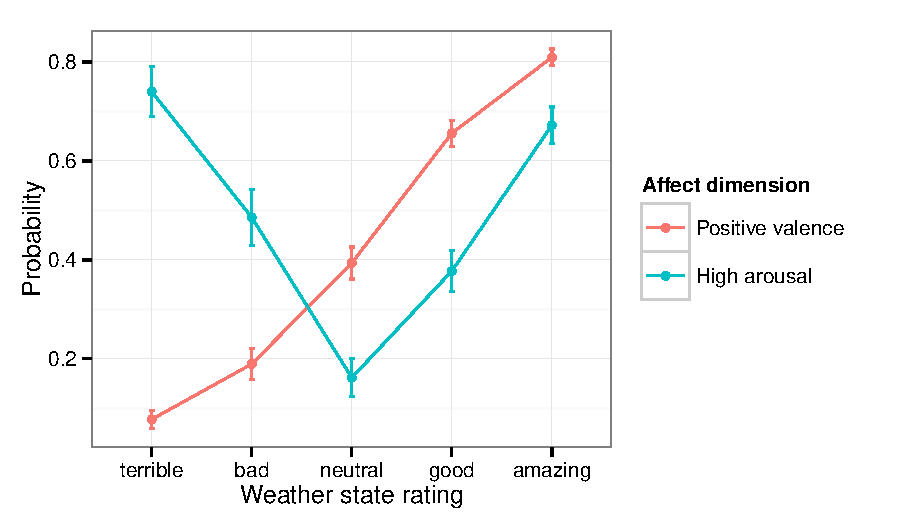
\includegraphics[width=220pt, height=130pt]{affect-prior.pdf}
\caption{The average probabilities of positive valence and high arousal associated with each weather state. Error bars are $95\%$ confidence intervals.}
\label{affect-prior}
\end{figure}

For each of the nine weather contexts, we obtained the number of participants who gave each of the weather state ratings and performed add-one Laplace smoothing on the counts. This allowed us to compute a smoothed prior distribution over weather states given each context, namely $P(s)$. Figure~\ref{priors} shows that the sunny and positive weather contexts were more likely to be rated as \texttt{amazing}, while the negative weather contexts were more likely to be rated as \texttt{bad} or \texttt{terrible}.  %\todo[inline]{RDH: obviously, need some way of identifying what the different rows and columns of the grid mean}

To examine participants' ratings of the affects associated with each context, we first performed Principal Component Analysis (PCA) on the seven emotion category ratings. This allowed us to compress the ratings onto a lower-dimensional space and reveal the main affective dimensions that are important in this domain. We found that the first two principal components corresponded to the dimensions of emotional valence and emotional arousal, accounting for $69.14\%$ and $13.86\%$ of the variance in the data, respectively.
%\todo{we should do a free response version of this task (``Ann feels ..... about the weather.''), before and after a statement, at some point to see if we are missing any affects... probably not needed for cogsci.}
The PCA represents emotion ratings for each trial as real values between negative and positive infinity on each of the dimensions. To map these values onto probability space, we first standardized the scores on each dimension to have zero mean and unit variance. We then used the cumulative distribution function to convert the standardized scores into values between $0$ and $1$. \todo{Necessary to say more?} This gives us the probabilities of Ann feeling positive valence and high arousal for each trial, which is a two-dimensional probabilistic representation of her affect.
%Although these values are treated as probabilities of a binary variable, they approximately track the \emph{degree} of positive valence and arousal as well; for example, $P(A_v) = 0.6$ suggests that the valence is more positive than neutral, and $P(A_a) = 0.1$ suggests that the arousal is quite low. 
By calculating the average probabilities of positive valence and high arousal given each weather state rating, we obtain the probability of positive valence and high arousal associated with each weather state, namely $P(A | s)$ (Figure ~\ref{affect-prior}).
%\todo[inline]{NDG: does this imply that valence and arousal are independent? they generally aren't.... i'm a bit confused about where the model's $A$ states fall with respect to the valence-arousal quadratic curve....}

%\todo{JTK: something about how this is not a perfect transformation but does approximately the right thing} 

%\begin{figure}
%\begin{minipage}[b]{.5\textwidth}
%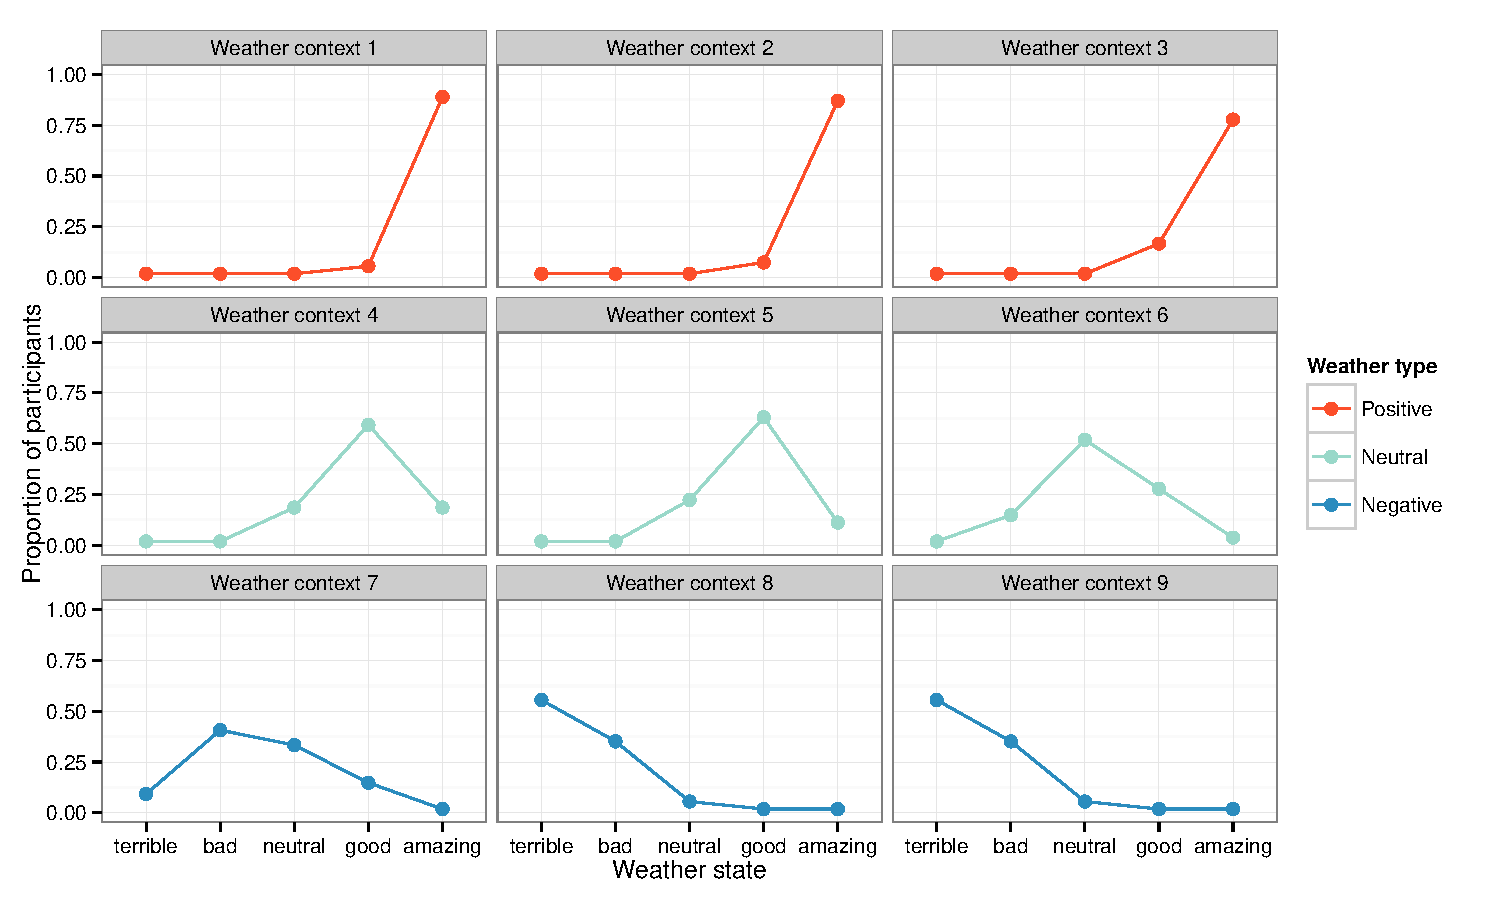
\includegraphics[width=5cm, height=3.7cm]{priors.pdf}
%\end{minipage}
%\begin{minipage}[b]{.4\textwidth}
%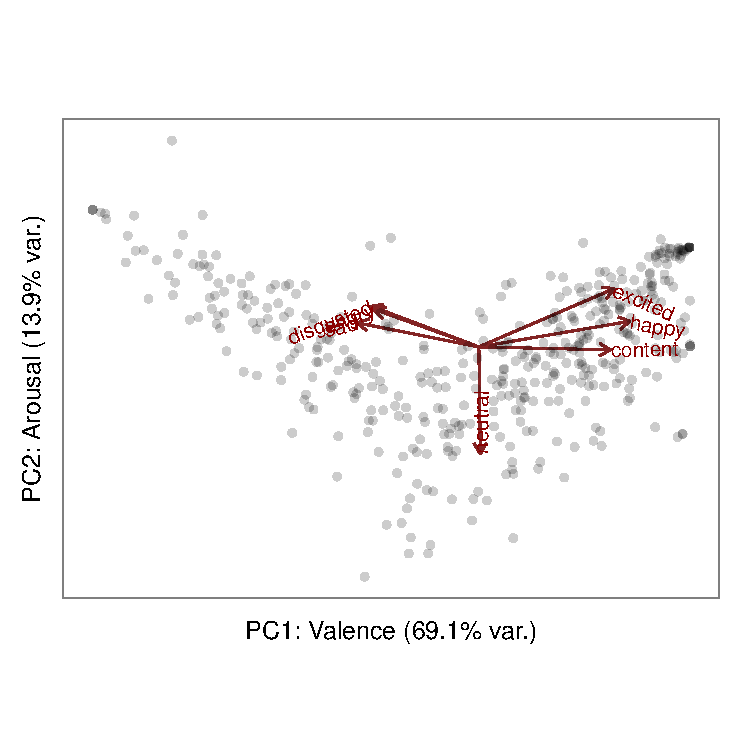
\includegraphics[width=5cm, height=5cm]{biplot.pdf}
%\end{minipage}
%
%\end{figure}

\begin{figure}[t]
\scalebox{0.38}{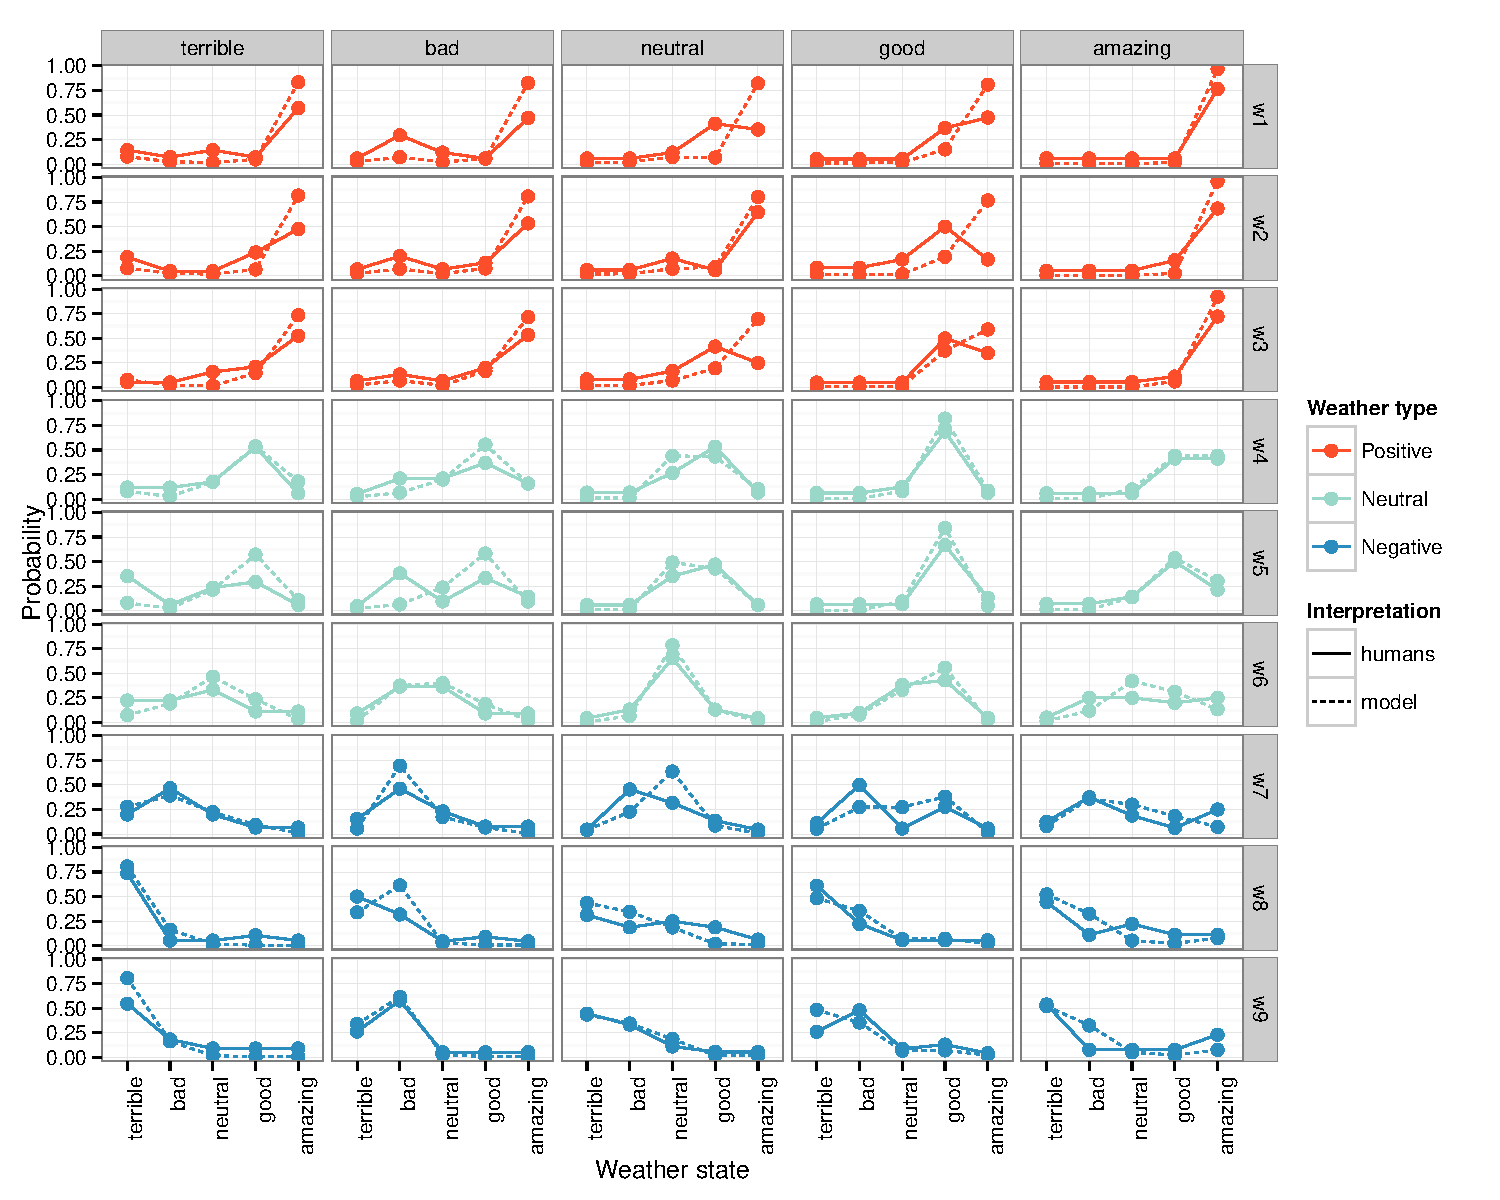
\includegraphics{model-state.pdf}}
\caption{Model's and participants' inferences about the weather state (x-axis) given a weather context (row) and an utterance (column). Each panel represents interpretations of an utterance in a weather context. The solid lines are participants' ratings; the dotted lines are model's posterior distributions over weather states.}
\label{model-state}
\end{figure}

\begin{figure*}[t]
\centering
\begin{subfigure}{0.4\textwidth}
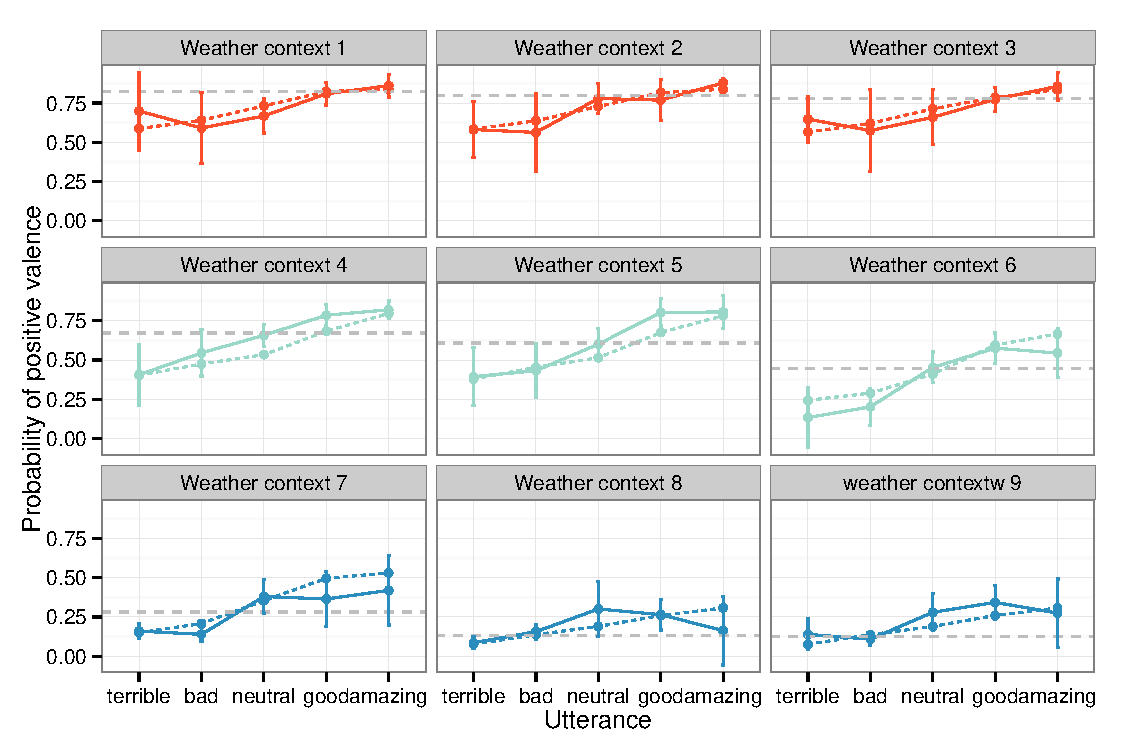
\includegraphics[width=200pt, height=140pt]{model-valence.pdf}
\caption{Average probabilities of speaker feeling positive valence given her utterance in a weather context.}
\label{valence}
\end{subfigure}
\begin{subfigure}{0.43\textwidth}
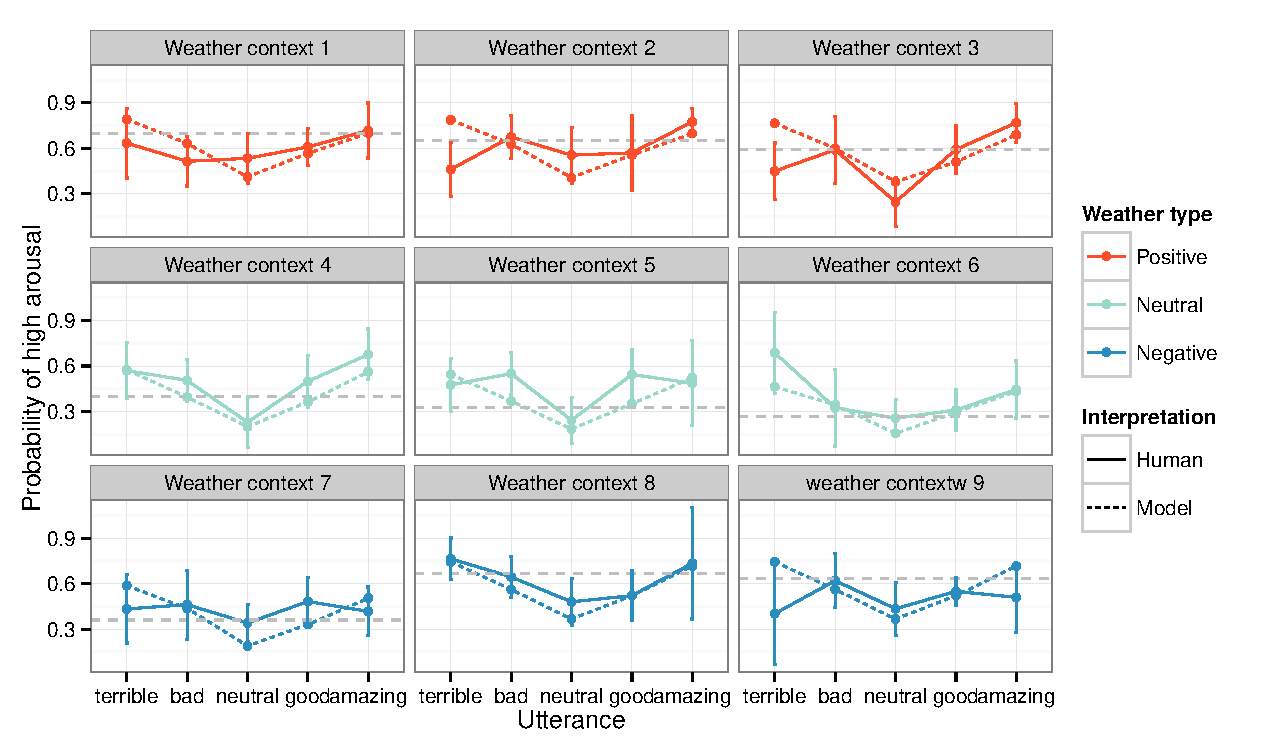
\includegraphics[width=220pt, height=140pt]{model-arousal.pdf}
\caption{Average probabilities of speaker feeling high arousal given her utterance in a weather context.}
\label{arousal}
\end{subfigure}
\begin{subfigure}{0.15\textwidth}
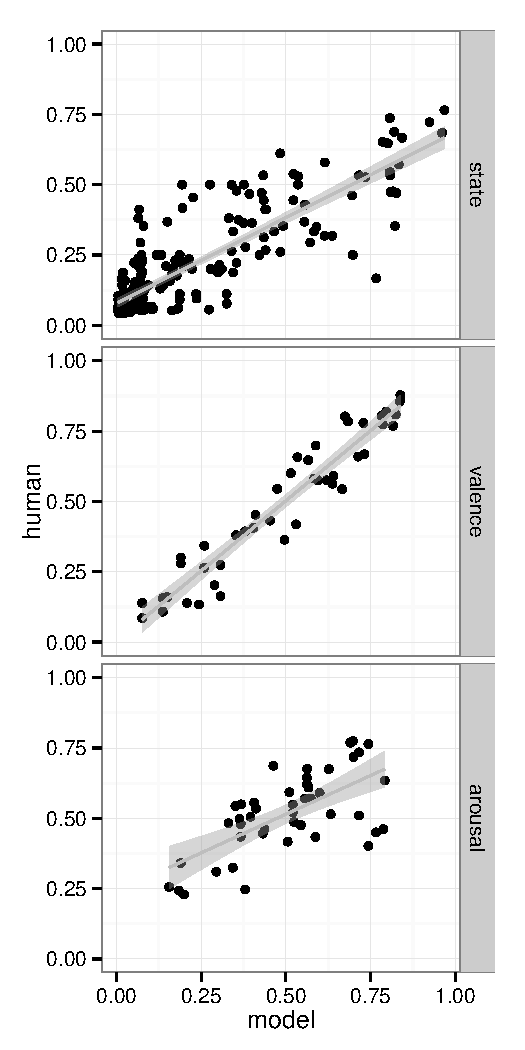
\includegraphics[width=75pt, height=140pt]{scatters.pdf}
\caption{Scatter plot of human versus model interpretations.}
\label{scatter}
\end{subfigure}
\end{figure*}


\subsection{Experiment 2: Irony understanding}
%In Experiment 1, we obtained the prior distribution over weather states for each weather context as well as the prior probabilities of positive valence and high arousal given each weather state. 
Results from Experiment 1 give us the components to generate interpretations of utterances from our model. Here we describe an experiment that elicits people's interpretations of utterances, which we then use to evaluate model predictions. 


\subsubsection{Materials and methods}
$59$ native English speakers with IP addresses in the United States were recruited on Amazon's Mechanical Turk. Each participant saw all nine images from Figure~\ref{images} in random order. In each trial, participants were told that a person (e.g. Ann) and her friend are in a room looking out the window together and see the view depicted by the image. Ann says, ``The weather is \underline{\hspace{1cm}}!" where the adjective is randomly selected at each trial from the following set: ``terrible," ``bad," ``ok," ``good," and ``amazing." Participants first rated how likely it is that Ann's statement is ironic using a slider with end points labeled ``Definitely NOT ironic" and ``Definitely ironic." They then indicated how Ann would actually rate the weather using a labeled 5-point Likert scale, ranging from \texttt{terrible}, \texttt{bad}, \texttt{neutral}, \texttt{good}, to \texttt{amazing}. Finally, participants used sliders to rate how likely it is that Ann feels each of seven emotions about the weather. A link to the experiment is here: \url{http://stanford.edu/~justinek/irony_exp/interpretation/interpretation_askIrony.html}

\subsubsection{Results}
We first examined participants' irony ratings for each of the weather context and utterance pairs. We found a basic irony effect, where utterances whose polarities are inconsistent with the polarity of the weather context are rated as significantly more ironic than utterances whose polarities are consistent with the weather context ($t(34.16)= -11.12, p < 0.0001$). For example, ``The weather is terrible" (a negative utterance) is rated as more ironic in weather context 1 (positive context) ($M = 0.90$, $SD = 0.21$) than in weather context 7 (negative context) ($M =0.15$,	$SD = 0.27$). A linear regression model with the polarity of the utterance, the polarity of the weather context, and their interaction as predictors of irony ratings produced an adjusted $R^{2}$ of 0.91, capturing most of the variance in the data. This suggests that participants' lay judgments of irony align with its basic definition: utterances whose apparent meanings are opposite in polarity to the speaker's intended meaning.

%We coded ``terrible" and ``bad" as \emph{negative} utterances, ``ok" as a \emph{neutral} utterance, and ``good" and ``amazing" as \emph{positive} utterances. We also coded each image as \emph{positive, neutral}, or \emph{negative} based on the modal weather state rating from Experiment 1 (e.g. $w_1$ is \emph{positive}, $w_6$ is \emph{neutral}, and $w7$ is \emph{negative}).

%\todo[inline]{RDH: I'm getting confused about utterance polarity vs. weather state polarity (possibly since they take on the same values), and this confusion compounded over the next paragraphs where you present more measures. Maybe lay this out in a way that distinguishes them better? Even putting ``utterance polarity'' and ``context polarity'' in bold font or something might help.}

Given the fact that participants can identify verbal irony based on its inconsistency with context, how do they then use context to determine the speaker's intended meaning? We examined participants' interpretations of utterances given contexts. For each of the $45$ weather context (9) $\times$ utterance (5) pairs, we obtained the number of participants who gave each of the five weather state ratings (\texttt{terrible, bad, neutral, good, amazing}). We performed add-one Laplace smoothing on the counts to obtain a smoothed distribution over weather states given each context and utterance. The solid lines in Figure~\ref{model-state} show these distributions of ratings. We see that participants produce ironic interpretations of utterances, such that the weather is most likely to be \texttt{amazing} given that the speaker said ``The weather is terrible" in weather context 1. Participants also produce hyperbolic interpretations, such that the weather is most likely to be \texttt{bad} given that the speaker said ``The weather is terrible" in weather context 7. This suggests that people are highly sensitive to context when interpreting utterances, and use it both to determine when an utterance is not meant literally and to appropriately recover the intended meaning. 

Finally, we examine participants' inferences about the speaker's affect given utterances in context. We used the loadings from the PCA on emotion ratings from Experiment 1 to project the emotion ratings from Experiment 2 onto the same dimensions. We then standardized and used the cumulative distribution function to convert the scores into values between $0$ and $1$. Figure ~\ref{valence} shows the average probability of \emph{positive valence} given an utterance in a weather context. The dotted gray lines are the average probabilities of positive valence associated with each weather context without any linguistic input, taken from Experiment 1. 
%
%We see that for the \emph{positive} weather contexts, the speaker is interpreted as more likely expressing positive valence given the extremely negative utterance ``terrible" than given the less negative utterance ``bad." On the other hand, for the \emph{negative} weather contexts, the speaker is interpreted as less likely expressing positive valence given the extremely positive utterance ``amazing" than the less positive utterance ``good" (STATS). This suggests that extreme utterances that are inconsistent with the valence of the context are more likely to express an opposite affect than its literal meaning.
%\todo[inline]{maybe you could use different names for the weather contexts? Like $\mathcal{W}_{neg}, \mathcal{W}_{neut}, \mathcal{W}_{pos}$, and then refer to $w_i \in \mathcal{W}_{neg}$ and so on.}
%
Figure ~\ref{arousal} shows the average probability of \emph{high arousal} given an utterance in a weather context. The dotted gray lines are the average probabilities of high arousal associated with each weather context without any linguistic input, taken from Experiment 1. 
%We see that regardless of the weather context, more extreme utterances (e.g. ``terrible" and ``amazing") are more likely to communicate high arousal.
%\todo[inline]{JTK: figure out data take-home point here}
%\todo{it's interesting that ``terrible'' seems to have suppressed arousal compared to ``bad''. any thoughts about why?}


%We call this distribution the \emph{interpreted meaning} of an utterance in context. We found that participants often rated the speaker (e.g. Ann) as judging the actual weather state to be different from what she described in her utterance, suggesting that participants interpreted these utterances non-literally. To further examine the relationship between literal meaning, interpreted meaning, and judgements of irony, we computed the Kullback-Leibler divergence between the literal interpretation of the utterance and the distribution over weather states given the context and utterance. 
%\todo{what is the literal distribution? if it's delta on the word corresponding state, then isn't KL just the interpretation log-prob of the state?}
%\todo[inline]{RDH: I don't quite understand what the KL divergence is measuring in the next paragraph}
%
%We found that adding the KL divergence measure to the linear regression model captured significantly more variance in the irony ratings, with an R-squared of 0.93 (more STATS). 
%\todo{this doesn't seem like the right analysis.... and a 1\% gain is pretty minimal to fuss about.} 


\section{Model Evaluation}
We now evaluate the model's performance against these behavioral results. From Experiment 1, we obtained the prior probability of a weather state given a context as well as the probability of affect given a weather state. In addition, we fit three free parameters to maximize correlation with data from Experiment 2: the speaker optimality parameter ($\lambda = 1)$ and the prior probability of each of the three QUDs ($P(q_{state}) = 0.3$, $P(q_{valence}) = 0.3$, $P(q_{arousal}) = 0.4$) \footnote{Since $P(q_{state}) + P(q_{valence}) + P(q_{arousal}) = 1$, $P(q_{arousal})$ is determined by the other two QUD parameters and does not count as a free parameter.}.
%\todo{NDG: the three QUD probs aren't independent, so only 3 free params, right?}  
For each of the $45$ utterance and weather context pairs, the model produced an interpretation consisting of the joint posterior distribution $P(s, A | u)$, where $A$ can be further broken down into valence and arousal dimensions. We will examine the model's performance on each of these state and affect dimensions by marginalizing over the other dimensions.

\todo[inline]{NDG: for each of these correlations also report percent of explainable variance captured with CI (footnote can explain what that is) JTK: still need to do this.}
Figure ~\ref{scatter} shows scatter plots correlating model predictions with human interpretation data for each of the dimensions: \textbf{state}, \textbf{valence}, and \textbf{arousal}. %Figure ~\ref{model-state} shows participants' and the model's inferences about the actual weather state given an utterance and a weather context. 
The model predictions closely match humans' interpretations, with a correlation of $0.86$. 
The model corresponds to humans' interpretations of valence extremely well, with a correlation of $0.96$. 
%Figure ~\ref{valence} shows participants' and the models' inference about the speaker's valence given an utterance and a weather context. From the tight correspondence between model and human interpretations of valence ($r=0.96$), we see that the model is able to incorporate the valence associated with the utterance's literal meaning (e.g. ``The weather is terrible") and the valence associated with the weather context (e.g. weather context 1) to interpret the probability of the speaker feeling positive valence. 
Importantly, the model infers the appropriate valence even when it is inconsistent with the valence of the utterance's literal meaning, thus capturing the essence of irony. 
%\todo{note that this is the case even when interpreted valence mismatches the prior expected valence given literal meaning -- i.e. the model captures irony in valence.}
The model's prediction for emotional arousal match humans' with a correlation of $0.66$. Furthermore, our model is able to use the inconsistent polarities between the context and utterance to predict people's irony ratings \todo{JTK: stats!}.
%Figure~\ref{arousal} shows participants' and the model's inferences about the speaker's arousal. 
%\todo{why is this correlation low? is it because of the terrible-bad inversion i asked about above?}

We describe a series of simpler models to show that the full model using a two-dimensional affect space best predicts human interpretations. We first examine a model that interprets utterances literally, such that ``The weather is terrible" is interpreted as the weather state being \texttt{terrible}, along with the valence and arousal associated with \texttt{terrible} weather. 
%Such a model produces a distribution over states that correlates with humans' interpretations with $r=0.38$, inference about valence that correlates with humans' with $r=0.45$, and inferences about arousal with a correlation of $r=0.49$. 
We then examine a model that simply ignores the speaker's utterance and takes into account only the state and affect priors associated with each weather context. 
%Such a model produces a distribution over states that correlates with humans' interpretations with $r=0.79$, inferences abut valence that correlate with $r=0.84$, and inferences about arousal that correlate with $r= 0.49$. 
Finally, we examine the performance of a qRSA model with the unidimensional affect space of valence. 
Table~\ref{table1} shows correlations with each dimension of the human data for each model.
A model that considers both affect and arousal QUDs outperforms the other models, especially with respect to inferences about valence, which is the most important aspect of irony.
These results suggest that by reasoning about a speaker who may want to communicate her emotional arousal in addition to valence, the model is able to incorporate background knowledge and linguistic information to produce the appropriate nonliteral interpretations---ironic and hyperbolic---as well as the associated affects. 
%Fitting two free parameters to maximize fit with human data, the model obtains a state correlation of $r=0.84$, a valence correlation of $r=0.79$, and an arousal correlation of $r=0.61$.

\begin{table}
\begin{tabular}{ |c | c | c | c | c | }
  \hline
  Model & State & Valence & Arousal & Average \\\hline                        
  Literal & 0.38 & 0.45 & 0.49 & 0.44\\
  Prior & 0.79 & 0.84 & 0.49 &  0.71 \\
  Valence & 0.84 & 0.79 & 0.61 & 0.75 \\
  Valence + arousal & 0.86 & 0.96 & 0.66 & 0.83\\
  \hline  
\end{tabular}
\caption{}
\label{table1}
\end{table}


%\todo[inline]{it would be nice to have some more direct analysis of irony -- that when state/valence mismatches that expected from literal meaning the model can predict it. this may also be a good place to come back to the explicit irony judgements: something like probability the interpretation is on the opposite side of the prior mean? or something more general that would also apply to ironic propositions? oh.. we should totally say something in the discussion about ironic propositions and other non-scalar irony.}

\section{Discussion}
%\todo[inline]{summary of take-home point}
In this paper, we explored the consequences of expanding the space of affect considered in Rational Speech Act models to account for verbal irony. We showed that by making a minimal extension to \citeA{kao2014nonliteral}'s hyperbole model, we can capture people's fine-grained interpretations of ironic utterances. The similarities between these models suggest that understanding hyperbole and irony requires the same underlying principles of communication, which aligns with other informal accounts of the pragmatics of nonliteral language understanding (cite).  

While we present evidence of shared communicative principles that unify irony and other forms of nonliteral language, there remain important qualities of verbal irony that may be unique. For example, the echoic mention theory of irony claims that speakers often use verbal irony to remind the listener of previous utterances that turned out to be false or irrelevant, or of positive norms that were explicitly violated \cite{sperber1981irony, jorgensen1984test}. On the other hand, pretense theory argues that when a speaker produces an ironic utterance, she is not genuinely making the utterance, but only pretending to be someone who would make such an utterance \cite{clark1984pretense}. 
%In this view, recognizing the pretense is central to interpreting verbal irony.
%The latter point in particular has interesting implications on the experiments we present here. While we asked participants to rate the speaker's affect given her utterance, it may be the case that the speaker is only \emph{pretending} to  
\todo{JTK: Say something about how terrible may involve pretense?} 
While our model so far does not explicitly incorporate elements of echoic mention or pretense, it is able to capture many of the main characteristics of verbal irony. By addressing these additional components in future research, we hope to further improve our model's performance and enrich its understanding of the social aspects of irony. 
\todo[inline]{JTK: say something about non-scalar irony?}

%\todo[inline]{connection to NLP}
In addition to shedding light on the communicative principles underlying irony understanding, our work also has interesting connections to natural language processing. Given the prevalence of irony in natural language, many researchers aim to automatically detect sarcasm in large bodies of texts in order to recover the correct sentiment from an ostensibly positive or negative utterance (e.g. ``I was overjoyed to pay $\$30$ for an overcooked steak") \cite{davidov2010semi, filatova2012irony}. A critical insight that emerged from these efforts is that irony detection requires information far beyond surface linguistic cues, often calling upon a deep understanding of context and common knowledge between speaker and listener that computers currently lack \cite{gonzalez2011identifying, wallacehumans}. By integrating background knowledge and linguistic meaning in a principled manner, we present a formal model that predicts ironic interpretations in a way that is highly sensitive to context and common ground. 

We believe that our experimental paradigm and modeling framework lend itself well to a more detailed and precise account of irony understanding. Given the prevalence of irony in everyday language and the social functions it serves, it would be \emph{amazing} (literally) to understand people's ability to use and interpret utterances that mean the opposite of what they say. 

%say the opposite of what they mean.
%
%Our experimental paradigm and modeling framework lends itself well to a more detailed and precise account of irony understanding. For example, what are the range of social and affective meanings involved in irony? How do people use irony to signal social closeness with the listener?
%


%. Indeed, without sufficient contextual information, even human beings exhibit poor judgment of verbal irony 

%\todo[inline]{future directions and conclusion}
%Our experimental paradigm and modeling framework lends itself well to a more detailed and precise account of irony understanding. For example, what are the range of social and affective meanings involved in irony understanding? We identified emotional valence and arousal in these experiments, but there may be others ....(attitudes? opinions? affect? social closeness?)
%(TODO: finish) What are the social functions of irony? Irony is often used to signal social closeness with the listener, presumably because it expresses the speaker's assumption that she and the listener share a great deal of common ground (cite). Given an ambiguous utterance that could be interpreted either literally or ironically, if a speaker supplements the utterance with prosodic cues to signal that it is meant ironically, will listeners judge the speaker as being closer to them? Can our model more directly  test the predictions of the echoic mention and pretense theories of irony and help distinguish between them? 




%A deeper point we wish to make with this work is that communication in general, and nonliteral language understanding in particular, relies on reasoning about the speaker's communicative goals during interpretation. Furthermore, these goals are often social or affective in nature, and speakers are adept at harnessing shared background knowledge with the listener to convey rich affective meanings without explicitly stating them. 
%
%\todo[inline]{relationship to hyperbole and what that says about figurative language understanding more generally}


%With our behavioral experiments, we presented results showing the fine-grained effects of background knowledge on people's interpretations of ironic utterances, and identified the main affective dimensions that are conveyed by irony. In addition, we presented a computational model that predicts peoples' interpretations of ironic utterances using general communicative principles. In effect, the model is able to tell when an utterance is meant to be literal or ironic, and when meant to be ironic, what types of affect the speaker intends to convey. By reasoning about the speaker's communicative goals, the model goes beyond the literal meaning of an utterance to infer the actual state of the world. In addition, it recovers important aspects of the speaker's affect about the situation and captures the social and affective uses of irony. Together, these results suggest that basic principles of communication---background knowledge and reasoning about informativeness with respect to the speaker's communicative goals---may be an important driver of irony understanding.

%\todo[inline]{the above paragraph is murky. the below maybe gets more at our take-away point: the approach in kao2914 extends immediately to additional non-literal uses, by more carefully considering the space of covert meanings that may be conveyed. in general re-work this conclusion to be sharper, and clearer about the main points.}


%\todo[inline]{RDH: AMAZING discussion (but seriously, I think all the pieces are here, and you make a lot of neat connections). Overall, I'm wondering if there's a way to reduce the number of figures? 8 figures seems like a lot for a 6 page paper, and I'm worried you won't have space, especially if you want to add more figures for the results and model evaluation section (I counted three ``Figure XX'' placeholders). I didn't get much from 6 and 7, but maybe I just didn't understand the result they were showing. And maybe Figure 4 isn't needed, since it depicts the usual `valence/arousal' PCA space? Fig 1 and 2 could be combined into a multicolumn fig... }

\bibliographystyle{apacite}

\setlength{\bibleftmargin}{.125in}
\setlength{\bibindent}{-\bibleftmargin}

\bibliography{irony}


\end{document}
